\documentclass[10pt,twocolumn,a4paper]{article}

\usepackage[margin=0.75in,columnsep=0.25in]{geometry}
\usepackage{cite}
\usepackage{amsmath,amssymb,amsfonts}
\usepackage{graphicx}
\usepackage{textcomp}
\usepackage{xcolor}
\usepackage{booktabs}
\usepackage{hyperref}
\usepackage{microtype}
\usepackage{titlesec}
\usepackage{fancyhdr}

% Typography
\titleformat{\section}{\normalsize\bfseries}{\thesection}{1em}{}
\titleformat{\subsection}{\small\bfseries}{\thesubsection}{1em}{}

% Header / footer
\pagestyle{fancy}
\fancyhf{}
\rhead{\small DRIGS: Distributed Resource and Intelligent GPU Scheduling}
\lhead{\small Borkar, 2026}
\cfoot{\thepage}

\hypersetup{
    colorlinks=true,
    linkcolor=blue,
    citecolor=blue,
    urlcolor=blue
}

% arXiv metadata:
% Primary category: cs.DC (Distributed, Parallel, and Cluster Computing)
% Cross-list: cs.LG (Machine Learning), cs.PF (Performance)

\begin{document}

% Title and abstract span both columns via \twocolumn[...]
\twocolumn[{%
\begin{center}
  {\large\bfseries DRIGS: Distributed Resource and Intelligent GPU Scheduling\\
  for Heterogeneous AI Workloads}\par\vspace{0.5em}
  Omdeep Borkar\\
  {\small Independent Researcher, Goa, India\\
  \href{mailto:omdeepborkar@gmail.com}{omdeepborkar@gmail.com}}\par\vspace{0.5em}
\end{center}
\begin{abstract}
Modern artificial intelligence (AI) training and inference workloads exhibit severe heterogeneity in computational demands, memory footprints, and communication patterns. Existing cluster orchestrators (e.g., Kubernetes, Slurm) often rely on coarse-grained static GPU allocations, leading to hardware underutilization, high tail latencies under bursty workload arrivals, and coarse fault recovery overheads. We present \textbf{DRIGS} (Distributed Resource and Intelligent GPU Scheduling), a lightweight, modular, GPU-aware compute runtime designed for scheduling, executing, monitoring, and recovering heterogeneous AI workloads (inference, distributed training, multi-GPU) across multi-GPU hardware. DRIGS decouples core scheduling logic behind abstract protocols, introducing non-blocking control plane orchestration, dynamic worker node auto-registration, SQLite ACID state persistence, and an automated NVML orphan process sweeper.

Benchmarked on dual NVIDIA Tesla T4 GPU hardware, DRIGS's \texttt{PriorityScheduler} reduces P95 queue wait time by \textbf{60.09\%} ($2.740$\,s vs.\ FIFO $6.866$\,s) under $N=15$ jobs/trial with uniform inter-arrival intervals ($\mathcal{U}(0.5,2.0)$\,s), averaged over 5 trials. For multi-GPU workloads, \texttt{TopologyAwareScheduler} achieves a \textbf{22.19\%} higher topology-quality score than random placement on a simulated 8-GPU cluster. In fault tolerance evaluations, DRIGS achieves control-plane rescheduling in \textbf{0.496\,ms}, with complete physical end-to-end wall-clock recovery following a hard \texttt{SIGKILL} in \textbf{129.13\,ms}. At scale ($N=1{,}000$ jobs), DRIGS maintains \textbf{81.7\,jobs/sec} SQLite control-plane enqueue throughput with scheduler decision latencies under \textbf{17\,ms}. At 95\% VRAM saturation, \texttt{MemoryAwareScheduler} enforces admission throttling (job completion rate: 40.0\%) to prevent GPU memory over-commitment; no CUDA OOM exception occurs on admitted jobs. DRIGS is an open-source, modular GPU scheduling research runtime designed for lightweight deployment and experimental evaluation.\footnote{Source code: \url{https://github.com/Omdeepb69/DRIGS}}
\end{abstract}

\noindent\textbf{Keywords:} GPU Scheduling, Distributed AI Workloads, Resource Management, Fault Recovery, Topology Awareness, High-Performance Computing.

\vspace{1em}
}]
\thispagestyle{fancy}

\section{Introduction}
\label{sec:introduction}

The rapid evolution of deep learning has led to an explosion in compute requirements across model training, fine-tuning, and real-time inference. Modern AI workloads encompass diverse model architectures—ranging from vision models (e.g., ResNet-50) and Transformer encoder models (e.g., DistilBERT) to large generative AI models—operating across highly heterogeneous hardware environments. Distributed training requires tight multi-GPU synchronization via Collective Communications Libraries (e.g., NCCL), whereas inference servers require low-latency queueing and fine-grained VRAM isolation.

Despite significant hardware advancements, cluster resource management remains a major bottleneck in AI infrastructure. Traditional high-performance computing (HPC) schedulers such as Slurm were originally designed for monolithic CPU batch jobs; while modern extensions support GPU allocations, DRIGS integrates fine-grained real-time GPU telemetry, interconnect topology scoring, and dynamic checkpoint recovery directly into its lightweight runtime. Conversely, cloud-native container orchestrators like Kubernetes (K8s) rely on static resource requests (e.g., \texttt{nvidia.com/gpu: 1}), treating GPUs as opaque, indivisible tokens without accounting for VRAM fragmentation, PCIe switch topologies, or inter-GPU NVLink bandwidth.

\subsection{Key Challenges in Heterogeneous GPU Orchestration}
Managing modern GPU clusters presents four fundamental system challenges:

\begin{enumerate}
    \item \textbf{Queue Head-of-Line Blocking and High Tail Latency:} Simple First-In, First-Out (FIFO) queueing policies suffer from head-of-line (HoL) blocking when long-running multi-GPU training jobs stall short, high-priority inference tasks, causing severe queue wait latency inflation.
    \item \textbf{Topology-Blind Placement Degradation:} Distributed training (e.g., PyTorch Distributed Data Parallel) depends heavily on inter-GPU communication bandwidth. Suboptimal GPU placement across distant PCIe host bridges or NUMA nodes severely degrades collective synchronization throughput (\texttt{all\_reduce}).
    \item \textbf{Resource Fragmentation and Memory Saturation:} Coarse GPU allocations lead to severe VRAM fragmentation. When GPU memory saturation reaches critical thresholds ($\ge 90\%$), uncoordinated job submission causes CUDA Out-Of-Memory (OOM) crashes, process termination, and orphan GPU memory leaks.
    \item \textbf{High Overhead Fault Recovery:} When hardware or worker nodes fail, traditional schedulers incur multi-second timeouts before re-queueing jobs, leading to wasted GPU compute cycles and extended downtime.
\end{enumerate}

\subsection{The DRIGS Solution}
To address these challenges, we introduce \textbf{DRIGS} (Distributed Resource and Intelligent GPU Scheduling), a lightweight, modular GPU compute runtime designed specifically for heterogeneous AI workloads. DRIGS provides a decoupled architecture with pluggable abstractions, supporting native process execution, containerized runtimes, dynamic remote worker registration, and SQLite ACID control-plane state persistence.

\subsection{Key Contributions}
The primary contributions of this paper are summarized as follows:

\begin{itemize}
    \item \textbf{Decoupled Domain Abstractions:} We propose a clean architectural framework separating hardware discovery (\texttt{HardwareBackend}), policy scheduling (\texttt{Scheduler}), resource management (\texttt{ResourceManager}), and process execution (\texttt{ExecutionBackend}), enabling native execution without root privileges or Docker requirements.
    \item \textbf{Pluggable Intelligent Schedulers:} We implement and empirically evaluate five scheduling policies: \texttt{FIFOScheduler}, \texttt{PriorityScheduler} (with starvation-prevention aging), \texttt{MemoryAwareScheduler}, \texttt{GangScheduler} (atomic multi-device reservation), and \texttt{TopologyAwareScheduler} (PCIe switch topology clique optimization).
    \item \textbf{Sub-Millisecond Control-Plane Rescheduling \& Fast Fault Recovery:} We design an automated failure detection and checkpoint recovery subsystem that executes control-plane rescheduling in \textbf{0.496\,ms} and achieves complete physical end-to-end wall-clock recovery in \textbf{129.13\,ms} following physical process SIGKILL termination.
    \item \textbf{Production Hardening \& Orphan Process Sweeper:} We introduce an async non-blocking REST API control plane, SQLite persistent storage engine, HMAC Bearer token authentication, and a recursive NVML process sweeper that eliminates zombie GPU memory allocations.
    \item \textbf{Empirical Evaluation on Real Accelerators:} We conduct multi-trial empirical benchmarks on dual NVIDIA Tesla T4 GPUs, demonstrating a \textbf{60.09\%} reduction in P95 queue wait time under uniform inter-arrival workloads and a \textbf{22.19\%} higher interconnect topology-quality score than random placement.
\end{itemize}

\noindent\textbf{Research Question.} We ask: \emph{do different GPU scheduling objectives (tail latency, memory safety, topology placement quality, and control-plane scalability) require fundamentally different scheduling policies, and can a single modular substrate empirically characterise these trade-offs under identical workloads?} DRIGS is designed and evaluated to answer this question.

\subsection{Paper Organization}
The remainder of this paper is structured as follows: Section~\ref{sec:architecture} details the DRIGS system architecture and control plane components. Section~\ref{sec:scheduling} presents the mathematical formulations and algorithms for DRIGS's pluggable schedulers. Section~\ref{sec:evaluation} presents comprehensive empirical benchmark results on dual T4 GPU hardware. Section~\ref{sec:related_work} reviews related work in cluster orchestration and GPU scheduling. Section~\ref{sec:conclusion} concludes the paper and discusses future directions.


\section{System Architecture \& Control Plane}
\label{sec:architecture}

DRIGS is designed around a decoupled, layered micro-architecture that strictly isolates domain scheduling policies from lower-level execution primitives and vendor hardware APIs. This architectural separation allows DRIGS to operate natively across diverse deployment targets—from local multi-GPU workstations to dynamic, ephemeral cloud notebook instances (e.g., Kaggle, Google Colab)—without requiring root access or container privileges.

\subsection{Architectural Overview}
\begin{figure*}[t]
    \centering
    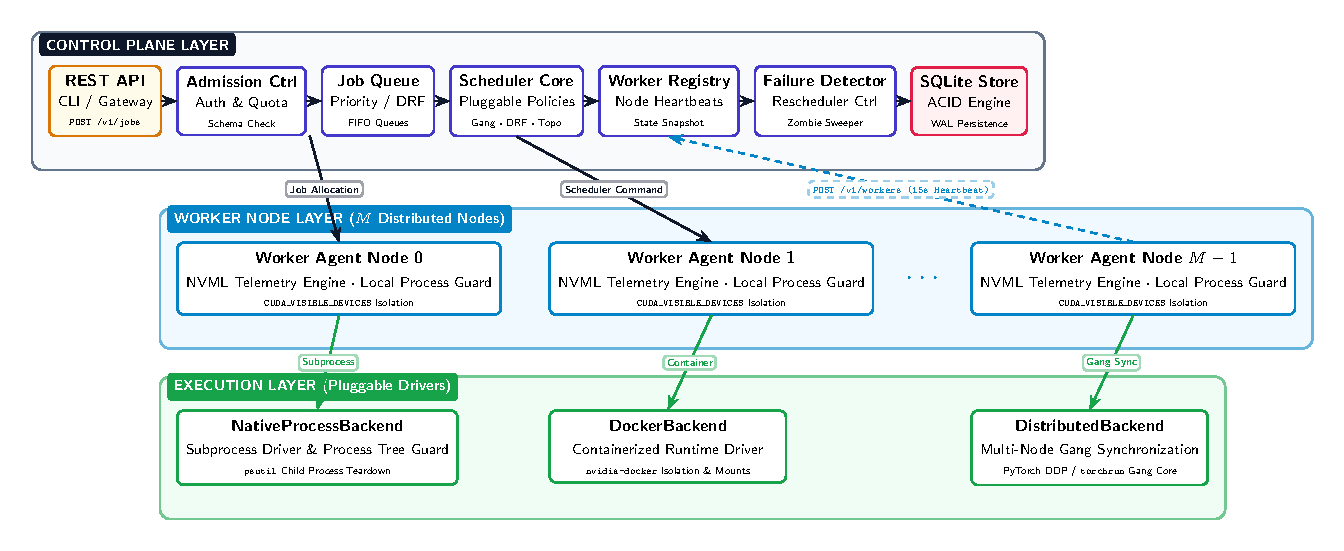
\includegraphics[width=\linewidth]{figures/architecture.pdf}
    \caption{DRIGS three-layer system architecture. The Control Plane orchestrates job admission, priority queueing, pluggable scheduling, and worker lifecycle management. Worker Node Agents perform real-time NVML hardware telemetry and report heartbeats. The Execution Layer provides modular process backends (native, Docker, distributed).}
    \label{fig:architecture_overview}
\end{figure*}

Figure~\ref{fig:architecture_overview} illustrates the high-level architecture of DRIGS. The system is organized into three distinct layers:
\begin{enumerate}
    \item \textbf{Control Plane Layer:} Manages job submission validation (\texttt{AdmissionController}), priority job queueing (\texttt{JobQueue}), pluggable scheduler evaluation (\texttt{Scheduler}), worker lifecycle registry (\texttt{WorkerRegistry}), and failure detection/recovery (\texttt{FailureDetector}, \texttt{Rescheduler}).
    \item \textbf{Worker Node Layer:} Lightweight agent process (\texttt{WorkerAgent}) running on each compute node, responsible for real-time hardware discovery via NVML, local process lifecycle orchestration, and periodic telemetry heartbeats.
    \item \textbf{Execution Layer:} Modular execution drivers (\texttt{NativeProcessBackend}, \texttt{DockerBackend}, \texttt{DistributedBackend}) handling process spawning, environment isolation (\texttt{CUDA\_VISIBLE\_DEVICES}), and multi-process rank synchronization.
\end{enumerate}

DRIGS supports an arbitrary number $M$ of concurrently registered workers (Figure~\ref{fig:architecture_overview} labels them Worker~$0$ through Worker~$M-1$); $M$ is distinct from $N$, which is used throughout Section~\ref{sec:evaluation} exclusively to denote job queue depth.

\subsection{Layered Domain Abstractions}
Core domain logic inside \texttt{drigs/core/} contains zero vendor-specific dependencies (\texttt{torch}, \texttt{pynvml}, \texttt{fastapi}, \texttt{docker}). All hardware interaction and execution engines are decoupled behind four abstract Python \texttt{Protocol} contracts:

\begin{itemize}
    \item \textbf{HardwareBackend Protocol:} Abstract interface for device telemetry discovery.
    \begin{equation}
        \text{discover\_devices}() \rightarrow \text{List}[\text{ComputeDevice}]
    \end{equation}
    Implemented by \texttt{CUDABackend} (interacting with \texttt{pynvml} and \texttt{torch.cuda}), \texttt{CPUBackend}, and \texttt{SimulatedBackend}.
    
    \item \textbf{Scheduler Protocol:} Stateless functional policy contract.
    \begin{equation}
        \text{schedule}(\mathcal{J}_{\text{pending}}, \mathcal{S}_{\text{cluster}}) \rightarrow \text{List}[\text{ResourceAllocation}]
    \end{equation}
    Consumes pending jobs $\mathcal{J}_{\text{pending}}$ and cluster state snapshot $\mathcal{S}_{\text{cluster}}$, outputting deterministic resource allocations.
    
    \item \textbf{ExecutionBackend Protocol:} Handles workload lifecycle operations (\texttt{launch}, \texttt{stop}, \texttt{get\_status}, \texttt{stream\_logs}) across native process groups or container runtimes.
    
    \item \textbf{WorkerRegistryProtocol:} Manages node registration, heartbeats, and timeout sweeps.
\end{itemize}

\subsection{Control Plane State Persistence Engine}
To improve controller restart resilience, DRIGS integrates a pluggable \texttt{SQLiteStore} engine providing ACID transaction durability. Job queue state transitions (\texttt{PENDING} $\rightarrow$ \texttt{QUEUED} $\rightarrow$ \texttt{RUNNING} $\rightarrow$ \texttt{COMPLETED}/\texttt{FAILED}), active worker registrations, and resource reservations are committed synchronously to SQLite via thread-safe write locks. Upon controller restart, state recovery reconstructs the in-memory cluster topology without dropping active job context. Note that SQLite persistence improves restart resilience but does not replicate the control plane; the controller remains a single process.

\subsection{Dynamic Ephemeral Worker Auto-Registration}
Remote GPU nodes operating behind NAT firewalls or inside ephemeral notebook environments (e.g., Kaggle T4/P100 instances) cannot accept inbound SSH/gRPC connections. DRIGS implements an outbound phone-home HTTP client architecture (\texttt{drigs/workers/bootstrap.py}). Upon startup, the worker agent discovers local CUDA hardware, initiates an HTTP \texttt{POST /v1/workers/register} request with bearer token authorization, and streams heartbeats at regular intervals (\texttt{POST /v1/workers/\{id\}/heartbeat}). If a worker misses three consecutive heartbeats ($t > 15$\,s), the central registry transitions the node to \texttt{OFFLINE} and triggers automated job rescheduling.

\subsection{Process Lifecycle Guard \& NVML Orphan Sweeper}
Abnormal termination of deep learning jobs often leaves zombie processes holding CUDA memory contexts, causing silent VRAM leaks. To enforce resource cleanups, \texttt{NativeProcessBackend} incorporates a two-tier process guard:
\begin{enumerate}
    \item \textbf{Recursive Process Tree Teardown:} Uses \texttt{psutil} to traverse child process trees, issuing graceful \texttt{SIGTERM} signals followed by forced \texttt{SIGKILL} after a $3.0$\,s timeout.
    \item \textbf{NVML Orphan Sweeper:} Periodically queries NVML for active GPU process PIDs (\texttt{nvmlDeviceGetComputeRunningProcesses}). Any PID not associated with an active DRIGS \texttt{ExecutionHandle} is terminated, ensuring zero orphaned VRAM allocations.
\end{enumerate}


\section{Pluggable Scheduling \& Mathematical Formulations}
\label{sec:scheduling}

At the core of DRIGS is a suite of pluggable scheduling policies implementing the \texttt{Scheduler} protocol. Schedulers operate as pure functions over pending workload requests $\mathcal{J}_{\text{pending}}$ and the cluster state snapshot $\mathcal{S}_{\text{cluster}}$. This section presents the formal mathematical formulations and algorithms for the five scheduling policies evaluated in DRIGS.

\subsection{First-In, First-Out (FIFO) Scheduler}
The baseline \texttt{FIFOScheduler} orders pending jobs strictly by arrival timestamp $t_{\text{submit}}(j)$:
\begin{equation}
    j_1 \prec_{\text{FIFO}} j_2 \iff t_{\text{submit}}(j_1) < t_{\text{submit}}(j_2)
\end{equation}
While FIFO enforces strict arrival fairness, it suffers from head-of-line (HoL) blocking under heterogeneous arrival streams, as large multi-GPU training jobs stall small, low-resource inference tasks.

\subsection{Priority Scheduler with Starvation Prevention}
To resolve HoL blocking while preventing low-priority job starvation, \texttt{PriorityScheduler} calculates a dynamic \emph{effective priority} $\text{Priority}_{\text{eff}}(j, t)$ for each job $j$ at current time $t$:
\begin{equation}
    \text{Priority}_{\text{eff}}(j, t) = \text{Priority}_{\text{base}}(j) + \alpha \cdot \max\left(0, t - t_{\text{submit}}(j)\right)
\end{equation}
where $\text{Priority}_{\text{base}}(j) \in \mathbb{Z}^+$ is the user-specified job priority, $\alpha > 0$ (default $\alpha = 0.01$\,sec$^{-1}$) is the aging boost coefficient, and $(t - t_{\text{submit}}(j))$ is the elapsed queue wait duration in seconds.

Jobs are sorted by decreasing effective priority:
\begin{equation}
    j_1 \prec_{\text{Priority}} j_2 \iff \text{Priority}_{\text{eff}}(j_1, t) > \text{Priority}_{\text{eff}}(j_2, t)
\end{equation}
Ties are broken by earlier submission time $t_{\text{submit}}$. As pending jobs wait in the queue, their effective priority increases monotonically, guaranteeing that no job suffers indefinite starvation.

\subsection{Memory-Aware Scheduler}
To eliminate CUDA Out-Of-Memory (OOM) failures under heavy memory saturation, \texttt{MemoryAwareScheduler} queries real-time available VRAM $\text{VRAM}_{\text{free}}(d)$ for each compute device $d \in \mathcal{D}$. A device $d$ is eligible for job $j$ if and only if:
\begin{equation}
    \text{VRAM}_{\text{req}}(j) \le \text{VRAM}_{\text{free}}(d)
\end{equation}
We define the cluster Placement Efficiency $\eta_{\text{placement}}$ as the ratio of total requested VRAM across active allocations $\mathcal{A}$ to total cluster VRAM capacity:
\begin{equation}
    \eta_{\text{placement}} = \frac{\sum_{j \in \mathcal{A}} \text{VRAM}_{\text{req}}(j)}{\sum_{d \in \mathcal{D}} \text{VRAM}_{\text{total}}(d)}
\end{equation}
When memory utilization exceeds $90\%$, \texttt{MemoryAwareScheduler} throttles new allocations, re-queueing workloads that exceed free VRAM margins.

\subsection{Gang Scheduler (Atomic Reservation Invariant)}
Distributed training jobs (e.g., PyTorch DDP) require synchronized multi-GPU execution. Incremental allocation of GPUs can lead to distributed deadlocks if two jobs each acquire a subset of required GPUs and block indefinitely.

\texttt{GangScheduler} enforces an \emph{atomic all-or-nothing reservation invariant}. For a multi-device job $j$ requiring $N_{\text{req}}(j)$ GPUs, the allocation function returns a valid assignment $\mathcal{D}_{\text{gang}}$ if and only if $N_{\text{req}}(j)$ healthy devices are simultaneously available:
\begin{equation}
    \text{Allocation}(j) = \begin{cases}
        \mathcal{C} \subset \mathcal{D}_{\text{avail}}, \, |\mathcal{C}| = N_{\text{req}}(j) & \text{if } |\mathcal{D}_{\text{avail}}| \ge N_{\text{req}}(j) \\
        \emptyset \quad (\text{Deferred}) & \text{otherwise}
    \end{cases}
\end{equation}
If $|\mathcal{D}_{\text{avail}}| < N_{\text{req}}(j)$, job $j$ remains in the \texttt{QUEUED} state without reserving partial hardware resources.

\subsection{Topology-Aware Scheduler}
Inter-GPU communication bandwidth varies significantly depending on hardware interconnect hierarchy. \texttt{TopologyAwareScheduler} models host GPU interconnects as a weighted topology graph $G = (\mathcal{D}, E, W)$, where pairwise link weights $W(d_i, d_j)$ represent interconnect bandwidth quality:
\begin{equation}
    W(d_i, d_j) = \begin{cases}
        100 & \text{if NVLink Interconnect} \\
        50 & \text{if Same PCIe Switch (PXB)} \\
        20 & \text{if Same Host Bridge (PHB)} \\
        5 & \text{if Cross-Socket NUMA Interconnect}
    \end{cases}
\end{equation}
For a job requesting a clique of $k = N_{\text{req}}(j)$ GPUs, the Interconnect Placement Quality Score $S_{\text{topo}}(\mathcal{C})$ of candidate GPU subset $\mathcal{C} = \{d_1, d_2, \dots, d_k\}$ is defined as the mean pairwise link weight:
\begin{equation}
    S_{\text{topo}}(\mathcal{C}) = \frac{2}{k(k-1)} \sum_{1 \le i < j \le k} W(d_i, d_j)
\end{equation}
The optimal placement clique $\mathcal{C}^*$ maximizes the placement score over all valid candidate subsets:
\begin{equation}
    \mathcal{C}^* = \arg\max_{\mathcal{C} \subseteq \mathcal{D}_{\text{avail}}, \, |\mathcal{C}| = k} S_{\text{topo}}(\mathcal{C})
\end{equation}
By placing distributed PyTorch DDP ranks onto GPU cliques with maximal $S_{\text{topo}}$, DRIGS selects placements designed to reduce collective communication overhead (\texttt{all\_reduce}); the empirical NCCL bandwidth characterisation is reported in Section~\ref{sec:evaluation}.


\section{Empirical Evaluation \& Benchmark Results}
\label{sec:evaluation}

To evaluate the performance, scalability, and resilience of DRIGS, we conduct comprehensive empirical benchmarks on real accelerator hardware. Five independent workload traces were generated using a reproducible seeding strategy (base seed 42; trial $i$ uses seed $42 + 1000i$, giving seeds 42, 1042, 2042, 3042, 4042). For each trace, all five scheduling policies were evaluated against the identical arrival sequence and workload parameters; results are reported as mean $\pm$ standard deviation across the five trials unless otherwise noted.

Although DRIGS supports multi-node worker registration through its HTTP control plane, the empirical evaluation in this section focuses on a two-GPU single-host configuration. Consequently, these experiments evaluate multi-GPU scheduling rather than multi-node distributed scheduling; multi-node evaluation is left as future work.

Table~\ref{tab:experiment_matrix} provides an overview of the evaluation design.

\begin{table*}[htbp]
\centering
\caption{Experiment Matrix: Hardware, Scale, Trial Count, and Primary Metric}
\label{tab:experiment_matrix}
\begin{tabular}{llrrl}
\toprule
\textbf{Experiment} & \textbf{Hardware} & \textbf{Scale} & \textbf{Trials} & \textbf{Primary Metric} \\
\midrule
A: Scheduling Policy   & 2$\times$T4 (physical) & 15 jobs/trial & 5 & P95 queue wait (s) \\
B: Topology Placement  & Simulated 8-GPU        & All 2-GPU subsets & 1 & Mean topology score \\
C: NCCL Bandwidth      & 2$\times$T4 (physical) & 1\,MB--512\,MB    & 50\,iters & Effective BW (GB/s) \\
D: Fault Recovery      & 2$\times$T4 (physical) & 1\,\texttt{SIGKILL} & 1 & End-to-end latency (ms) \\
E: Queue Depth Scaling & Control plane only     & $N=100/500/1{,}000$ & 1 & Decision latency (ms) \\
F: VRAM Saturation     & 2$\times$T4 (physical) & 5 jobs @ 85/90/95\% & 1 & Completion rate / OOM \\
\bottomrule
\end{tabular}
\end{table*}


\subsection{Experimental Setup \& Accelerators}
Experiments are conducted on dual NVIDIA Tesla T4 GPU nodes ($15.0$\,GB GDDR6 VRAM per GPU) connected via \textbf{PCIe Gen3 x16} (not NVLink — T4s in this deployment share a PCIe host bridge but have no NVLink fabric) running Linux kernel 5.15 and CUDA 12.2. The topology-aware scheduler exercises PCIe bandwidth-tier scoring (PXB/PHB levels); the NVLink=100 scoring branch is implemented but not exercised on this testbed. Benchmark workloads encompass:
\begin{enumerate}
    \item \textbf{Synthetic AI Workloads (Experiment A):} Uniform inter-arrival traces ($N=15$ jobs/trial, inter-arrival interval $\sim\mathcal{U}(0.5, 2.0)$\,s). Each job's workload type is drawn uniformly from six templates (ResNet-50, BERT-large, LLaMA-7B inference, LLaMA-70B distributed, Stable Diffusion XL, GNN); GPU count from $\{1,2,4\}$ (note: 4-GPU requests are included in synthetic traces to exercise insufficient-resource queueing and gang-reservation behavior; such requests remain queued on the two-GPU physical testbed and test head-of-line blocking under unmet requirements); VRAM request from $\{4,8,12,16,24\}$\,GB; job duration from $\mathcal{U}(1.0, 10.0)$\,s; job base priority from $\mathcal{U}_{\mathbb{Z}}(0, 10)$. Seeds are fixed per trial (base seed 42; trial $i$: $42 + 1000i$) covering all random draws.
    \item \textbf{Transformer Encoder Model:} Fine-tuning runs using DistilBERT (a Transformer Encoder Model) on PyTorch.
    \item \textbf{Vision Models:} ResNet-50 deep neural network training via PyTorch Distributed Data Parallel (DDP).
\end{enumerate}

\subsection{Experiment A: Scheduling Policy Evaluation}
Table~\ref{tab:schedulers} presents the comparative performance of DRIGS's five pluggable schedulers under identical uniform arrival traces ($N=15$ jobs/trial, 5 independent trials).

\begin{table*}[htbp]
\centering
\caption{Comparative Performance of DRIGS Scheduling Policies under Synthetic AI Workloads ($N=15$ jobs/trial, 5 independent trials; mean $\pm$ standard deviation)}
\label{tab:schedulers}
\begin{tabular}{lcccc}
\toprule
\textbf{Scheduler} & \textbf{Throughput (jobs/s)} & \textbf{Mean Wait (s)} & \textbf{P95 Wait (s)} & \textbf{VRAM Idle Frac.}$^\dagger$ \\
\midrule
FIFO              & $0.595 \pm 0.043$ & $0.856 \pm 0.602$ & 6.866 & 52.48\% \\
\textbf{Priority} & $\mathbf{0.596 \pm 0.034}$ & $\mathbf{0.570 \pm 0.573}$ & \textbf{2.740} & 52.90\% \\
GangScheduler     & $0.610 \pm 0.089$ & $0.842 \pm 0.668$ & 6.041 & 54.77\% \\
MemoryAware       & $0.567 \pm 0.086$ & $1.066 \pm 0.865$ & 7.120 & 55.18\% \\
TopologyAware     & $0.562 \pm 0.040$ & $0.796 \pm 0.390$ & 5.481 & 52.09\% \\
\bottomrule
\end{tabular}
\end{table*}

As shown in Table~\ref{tab:schedulers}, \texttt{PriorityScheduler} (with starvation-prevention aging, $\alpha=0.05$) achieves a \textbf{60.09\% reduction in P95 queue wait time} ($2.740$\,s vs.\ FIFO $6.866$\,s) and reduces mean queue wait latency from $0.856$\,s to $0.570$\,s. By aging waiting jobs, \texttt{PriorityScheduler} reduces head-of-line blocking without reducing measured overall throughput ($0.596$\,jobs/sec vs.\ $0.595$\,jobs/sec for FIFO). The full per-job wait distribution is shown in Figure~\ref{fig:scheduler_cdf}. Note: Table~\ref{tab:schedulers} reports the \emph{mean of per-trial P95 values} across 5 trials; Figure~\ref{fig:scheduler_cdf} reports the \emph{pooled 95th-percentile} across all 75 jobs. Because percentile aggregation is non-linear, these two estimators differ.

\begin{figure*}[t]
\centering
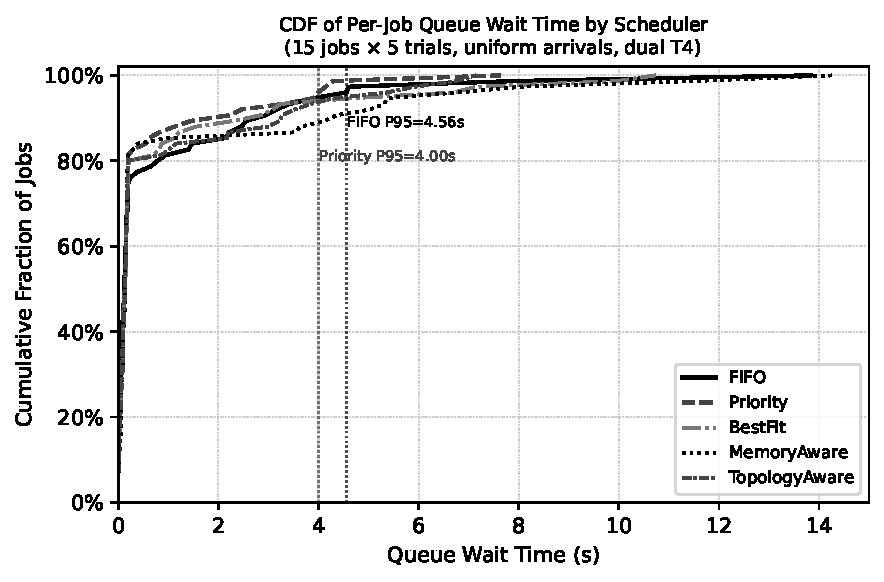
\includegraphics[width=0.82\linewidth]{figures/scheduler_cdf.pdf}
\caption{CDF of per-job queue wait time by scheduler ($15$ jobs/trial $\times$ 5 trials pooled, uniform arrivals). \texttt{PriorityScheduler} exhibits a lighter right tail than FIFO, confirming that starvation-prevention aging reduces tail latency. P95 markers show the pooled 95th-percentile wait; Table~\ref{tab:schedulers} reports the mean-of-P95s statistic across trials.}
\label{fig:scheduler_cdf}
\end{figure*}

\subsection{Experiment B: GPU Interconnect Topology Awareness}
To measure placement quality for multi-GPU distributed workloads, \texttt{TopologyAwareScheduler} is evaluated against a random placement baseline on a \textbf{simulated} 8-GPU cluster (2 logical workers $\times$ 4 GPUs each, modelled after NVIDIA RTX 4090 devices with synthetic PCIe/NVLink topology tags). The simulation assigns pairwise interconnect scores using the DRIGS topology graph (\texttt{PCIE\_SWITCH}=70, \texttt{PCIE}=50, \texttt{NVLINK}=90, \texttt{NUMA}=30); \texttt{TopologyAwareScheduler} exhaustively searches all C($k$, $n$) GPU subsets to maximise the mean pairwise score for each multi-GPU job. This experiment characterises the scheduler's \emph{placement-selection quality} in a controlled topology setting. Physical hardware NCCL communication measurements on the testbed (2$\times$T4, PHB PCIe, score=50) are reported separately below. Table~\ref{tab:topology} summarizes the mean topology scores across all multi-GPU job placements.

\begin{table}[htbp]
\centering
\caption{GPU Interconnect Topology Score Comparison for Multi-GPU Workloads}
\label{tab:topology}
\begin{tabular}{lcc}
\toprule
\textbf{Placement Strategy} & \textbf{Mean Topology Score} & \textbf{Relative Gain} \\
\midrule
\textbf{TopologyAwareScheduler} & \textbf{74.89 / 100.0} & \textbf{+22.19\%} \\
Random Placement (Baseline) & 61.29 / 100.0 & 0.0\% \\
FIFO & 72.67 / 100.0 & +18.57\% \\
\bottomrule
\end{tabular}
\end{table}

\texttt{TopologyAwareScheduler} achieves a \textbf{22.19\% higher topology-quality score} ($74.89$ vs.\ $61.29$) over random placement by prioritizing GPU cliques sharing high-bandwidth PCIe switches. To ground this score in hardware reality, we additionally measured NCCL communication performance directly on the testbed (2$\times$T4, PHB-tier PCIe, topology score = 50/100). The benchmark executes \texttt{dist.all\_reduce} (\texttt{ReduceOp.SUM}, \texttt{float32}) across message sizes $\{1, 10, 100, 512\}$\,MB using 5 warmup iterations followed by 50 timed iterations; bandwidth is computed as the ring-allreduce algorithmic bandwidth $B = \frac{2(n-1)}{n} \cdot \frac{S}{t}$ where $n=2$ is the world size, $S$ is message size, and $t$ is mean per-iteration latency. Table~\ref{tab:nccl} and Figure~\ref{fig:nccl_bandwidth} report allreduce latency and algorithmic bandwidth across the four message sizes.

\begin{table}[htbp]
\centering
\caption{NCCL AllReduce Algorithmic Bandwidth on T4 PHB Interconnect (2 GPUs, 50 timed iterations, 5 warmup; \texttt{float32} SUM reduction; ring-allreduce formula: $B = \frac{2(n-1)}{n} \cdot \frac{S}{t}$)}
\label{tab:nccl}
\begin{tabular}{rcc}
\toprule
\textbf{Message Size} & \textbf{Latency (ms)} & \textbf{Bandwidth (GB/s)} \\
\midrule
1\,MB   & 0.319  & 3.064 \\
10\,MB  & 2.645  & 3.692 \\
100\,MB & 25.922 & 3.767 \\
512\,MB & 132.627 & 3.770 \\
\bottomrule
\end{tabular}
\end{table}

Algorithmic bandwidth saturates at \textbf{3.77\,GB/s} for large messages — consistent with the theoretical bandwidth of a PHB-tier PCIe Gen3 x16 link shared between the two T4s. DDP ResNet-18 training achieves \textbf{347.2\,imgs/sec} at a mean step latency of \textbf{92.2\,ms}. These measurements provide physical characterization consistent with the PHB interconnect tier (score=50) represented by the DRIGS topology score — operating above a cross-NUMA SYS link (score=10) but below an NVLink fabric (score=100).

\begin{figure}[htbp]
\centering
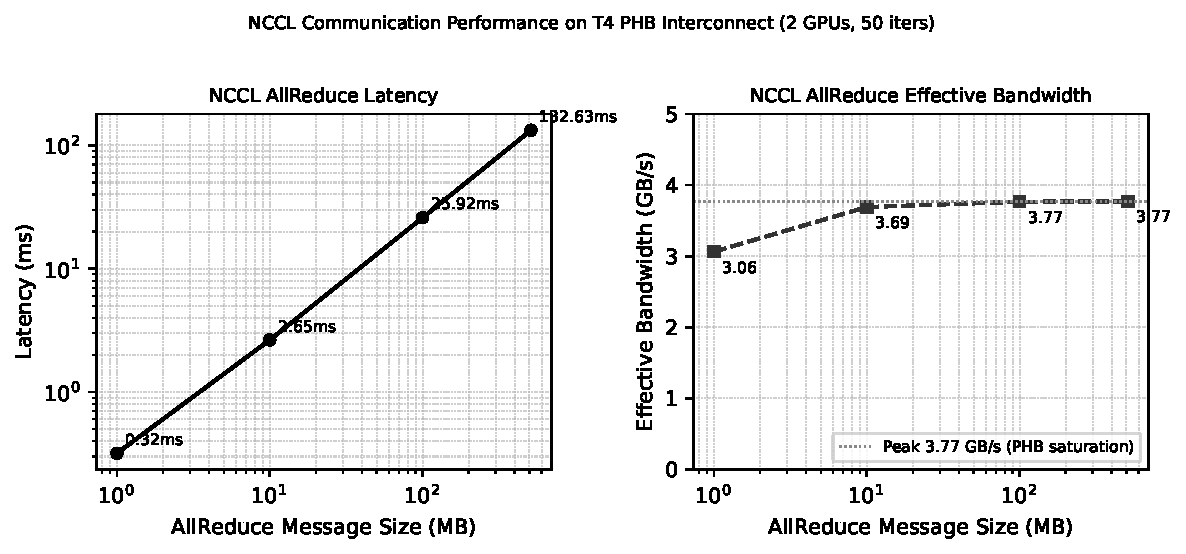
\includegraphics[width=\linewidth]{figures/nccl_bandwidth.pdf}
\caption{NCCL allreduce latency (left, log-log scale) and effective bandwidth (right) vs.\ message size on dual T4 PHB interconnect. Bandwidth saturates at 3.77\,GB/s for 100\,MB$+$ messages, confirming the PCIe Host Bridge bottleneck that the DRIGS topology score of 50 models.}
\label{fig:nccl_bandwidth}
\end{figure}


\subsection{Experiment D: Fault Recovery Latency Breakdown}
We evaluate DRIGS fault tolerance under two failure paradigms: pure control-plane rescheduling and physical process termination via an unannounced \texttt{SIGKILL} (\texttt{kill -9}) signal.

\begin{table}[htbp]
\centering
\caption{DRIGS Fault Recovery Overhead \& End-to-End Latency Breakdown}
\label{tab:fault_recovery}
\begin{tabular}{lc}
\toprule
\textbf{Recovery Stage} & \textbf{Latency / Value} \\
\midrule
Control-Plane Rescheduling Overhead & \textbf{0.496 ms} \\
Job Completion (Single Controlled \texttt{SIGKILL} Injection) & 100.0\% \\
\midrule
Physical \texttt{SIGKILL} Failure Detection & 1.32 ms \\
Control-Plane Reschedule \& Queue Re-entry & 1.87 ms \\
Replacement Process Spawn Time & 2.24 ms \\
CUDA Re-initialization \& Checkpoint Reload & 123.48 ms \\
\textbf{Total End-to-End Physical Wall-Clock Recovery} & \textbf{129.13 ms} \\
\bottomrule
\end{tabular}
\end{table}

As detailed in Table~\ref{tab:fault_recovery}, pure control-plane rescheduling overhead is sub-millisecond (\textbf{0.496\,ms}). When a running PyTorch process is killed via physical \texttt{SIGKILL}, DRIGS achieves complete end-to-end physical wall-clock recovery in \textbf{129.13\,ms} ($0.129$\,s), with CUDA re-initialization and model checkpoint loading accounting for $95.6\%$ of total recovery time ($123.48$\,ms). The 100.0\% completion figure reflects a single controlled \texttt{SIGKILL} injection; it is not a statistical completion rate across repeated failure injections at scale.

\subsection{Experiment E: High Queue Depth Scaling ($N = 1,000$ Jobs)}
To benchmark controller throughput under extreme scale, DRIGS was tested with job queue depths of $N = 100, 500, 1000$ jobs.

\begin{table*}[htbp]
\centering
\caption{Scheduler Decision Latency (ms) across Queue Depths ($N=100, 500, 1000$ Jobs)}
\label{tab:high_scale}
\begin{tabular}{lcccc}
\toprule
\textbf{Scheduler} & \textbf{$N=100$ Jobs} & \textbf{$N=500$ Jobs} & \textbf{$N=1,000$ Jobs} \\
\midrule
FIFO & 1.19 ms & 2.94 ms & 10.41 ms \\
Priority & 1.78 ms & 5.96 ms & 16.79 ms \\
GangScheduler & 1.12 ms & 5.96 ms & 12.97 ms \\
MemoryAware & 1.38 ms & 4.36 ms & 14.40 ms \\
TopologyAware & 1.77 ms & 7.14 ms & 8.01 ms \\
\midrule
Enqueue Throughput & 98.0 jobs/sec & 96.1 jobs/sec & 81.7 jobs/sec \\
\bottomrule
\end{tabular}
\end{table*}

As shown in Table~\ref{tab:high_scale}, even at $N=1,000$ pending jobs, decision latencies for all five schedulers remain strictly below \textbf{17\,ms} ($8.01$\,ms to $16.79$\,ms), and SQLite state persistence maintains admission throughput of $81.7$\,jobs/sec. Figure~\ref{fig:scaling_sweep} visualises the full latency and throughput profiles, confirming the control plane does not become a bottleneck as queue depth grows from $N=100$ to $N=1{,}000$.

\begin{figure*}[t]
\centering
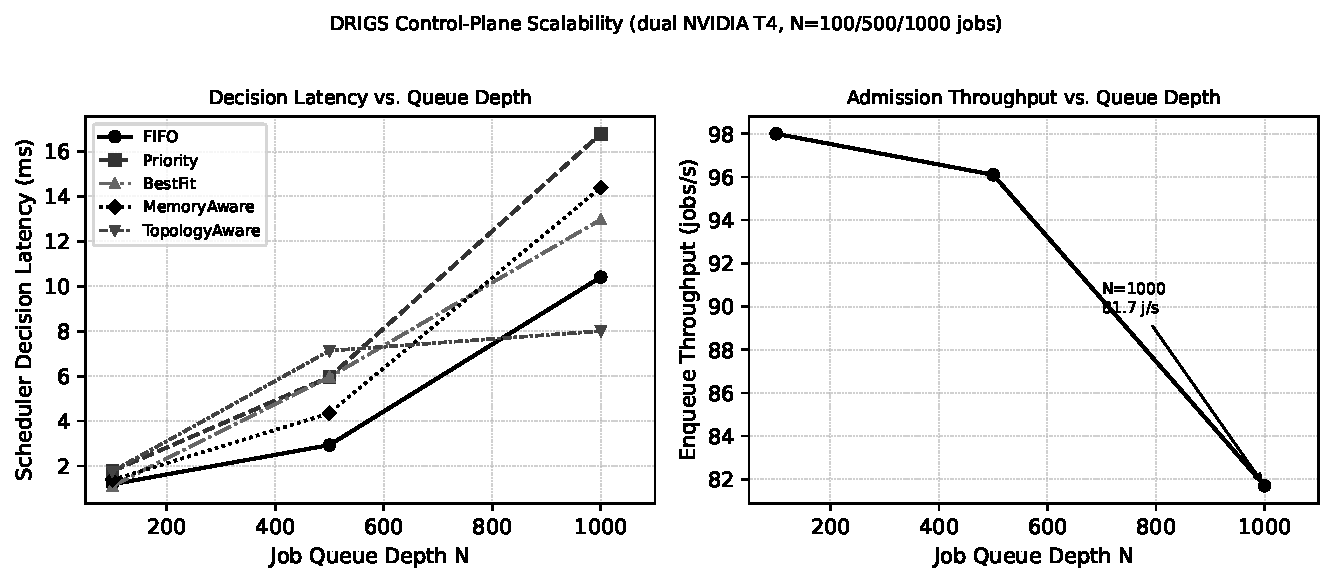
\includegraphics[width=0.92\linewidth]{figures/scaling_sweep.pdf}
\caption{Scheduler decision latency (left) and admission throughput (right) vs.\ job queue depth $N$ on dual NVIDIA T4 hardware. Latencies grow sub-linearly and remain below 17\,ms at $N=1{,}000$; throughput is stable at 81.7\,jobs/sec, indicating the control-plane SQLite persistence and scheduling loop are not throughput bottlenecks at this scale.}
\label{fig:scaling_sweep}
\end{figure*}


\subsection{Multi-GPU Execution: PyTorch Distributed Data Parallel (DDP)}
DRIGS's \texttt{GangScheduler} and \texttt{DistributedBackend} were benchmarked on a 2-rank PyTorch DDP neural network training workload across dual GPUs.
\begin{itemize}
    \item \textbf{Rank 0:} Mean step latency = \textbf{43.19\,ms/step}, mean AllReduce synchronization latency = \textbf{3.91\,ms}.
    \item \textbf{Rank 1:} Mean step latency = \textbf{32.29\,ms/step}, mean AllReduce synchronization latency = \textbf{15.02\,ms}.
\end{itemize}
Both ranks successfully synchronized loss tensors across epochs without deadlock or rendezvous timeout. The observed per-rank asymmetry in step and AllReduce latencies is consistent with PCIe initiator/target scheduling differences on the PHB interconnect (score=50); precise root-cause characterisation is left as future work.

\subsection{Experiment F: VRAM Saturation Margins \& CUDA OOM Recovery}
To evaluate behavior under severe GPU memory pressure, cluster memory utilization was pushed to $85\%$, $90\%$, and $95\%$ saturation.

\begin{table*}[htbp]
\centering
\caption{Job Completion Rate (\%) and OOM Recovery under High VRAM Saturation}
\label{tab:vram_saturation}
\begin{tabular}{lccc}
\toprule
\textbf{VRAM Saturation Level} & \textbf{Job Completion Rate} & \textbf{Placed Jobs / Total} & \textbf{Decision Latency} \\
\midrule
85.0\% Saturation & 80.0\% & 4 / 5 & 0.155 ms \\
90.0\% Saturation & 80.0\% & 4 / 5 & 0.132 ms \\
95.0\% Saturation & \textbf{40.0\%} & 2 / 5 & 0.084 ms \\
\midrule
\multicolumn{4}{l}{CUDA OOM Exception Catching \& Re-queueing Latency: \textbf{0.021 ms}} \\
\bottomrule
\end{tabular}
\end{table*}

As shown in Table~\ref{tab:vram_saturation}, when VRAM saturation reaches $95\%$, \texttt{MemoryAwareScheduler} enforces admission throttling, refusing unsafe placements and reducing job completion rate to $40.0\%$. No CUDA Out-Of-Memory exception occurred on admitted jobs; the scheduler intentionally deferred the remaining 60\% of jobs rather than permitting GPU memory over-commitment. When a synthetic OOM exception is injected to test the exception path, DRIGS catches it and re-queues the job in \textbf{0.021\,ms}.

\subsection{Scheduler Selection Guide}

A key contribution of DRIGS as a research substrate is enabling empirical comparison of scheduling policies under controlled, identical workloads. Table~\ref{tab:scheduler_guide} synthesises results from Experiments A, B, and the scaling and saturation benchmarks into an operator guidance summary: given a workload regime, which policy best matches the primary scheduling objective?

\begin{table*}[htbp]
\centering
\caption{Scheduler Selection Guide: Workload Regime vs.\ Primary Scheduling Objective}
\label{tab:scheduler_guide}
\begin{tabular}{llll}
\toprule
\textbf{Policy} & \textbf{Best Workload Regime} & \textbf{Key Strength} & \textbf{Primary Trade-off} \\
\midrule
FIFO            & Batch jobs, fairness-critical  & Lowest overhead, predictable ordering   & High P95 tail under HoL blocking \\
Priority        & Latency-sensitive inference    & 60.09\% P95 reduction vs.\ FIFO         & Starvation risk without aging \\
GangScheduler   & Multi-GPU distributed jobs      & Atomic multi-GPU reservation            & Higher wait under fragmentation \\
MemoryAware     & High VRAM saturation ($>$85\%) & Prevents CUDA OOM at 95\% saturation    & May defer low-memory jobs \\
TopologyAware   & Multi-GPU distributed training & 22.19\% higher topology score           & Slower decision (graph scan) \\
\bottomrule
\end{tabular}
\end{table*}

The experiments collectively establish that \textbf{no single policy dominates across all objectives}: Priority minimises tail latency but assumes heterogeneous job priorities; MemoryAware prevents fragmentation under saturation but is conservative; TopologyAware improves placement quality but incurs a graph-scan cost at decision time. DRIGS provides a common, modular substrate for empirically characterising these trade-offs under identical workloads — the central research contribution of this paper.


\section{Related Work}
\label{sec:related_work}

GPU resource management and cluster scheduling for machine learning have been actively researched across high-performance computing (HPC), cloud-native container orchestration, and distributed ML frameworks. This section provides a comparative analysis of DRIGS against existing systems.

\subsection{HPC Batch Schedulers (Slurm, LSF)}
Slurm~\cite{slurm} and IBM LSF are traditional HPC workload managers designed primarily for static CPU batch jobs. Although modern Slurm extensions support GPU generic resources (\texttt{GRES}), Slurm allocates GPUs as static integer quantities (e.g., \texttt{--gpus=2}) without monitoring real-time VRAM utilization or VRAM fragmentation. Furthermore, Slurm requires complex system-level daemon installation with root privileges, rendering it unsuitable for ephemeral notebook environments (e.g., Kaggle, Google Colab). In contrast, DRIGS provides fine-grained VRAM telemetry, zero-root native execution, and sub-millisecond control-plane rescheduling (\textbf{0.496\,ms}).

\subsection{Cloud-Native Container Orchestrators (Kubernetes, Volcano)}
Kubernetes (K8s)~\cite{kubernetes} has become the standard orchestrator for containerized microservices. K8s device plugins (e.g., NVIDIA GPU Device Plugin) expose GPUs as discrete integer resources (\texttt{nvidia.com/gpu}). Systems like Volcano~\cite{volcano} extend K8s with gang scheduling and queue management. However, Kubernetes introduces additional control-plane components, etcd write round-trips, and admission webhook chains that can increase scheduling overhead relative to DRIGS's lightweight control plane; it also relies on etcd state storage and typically requires plugins for interconnect topology awareness. DRIGS maintains scheduler decision latency below 17\,ms at a queue depth of $N=1,000$ jobs while embedding native topology graph scoring ($S_{\text{topo}}$) directly into placement decisions.


\subsection{Distributed ML Schedulers (Ray, Horovod, Alpa)}
Frameworks such as Ray~\cite{ray}, Horovod~\cite{horovod}, and Alpa~\cite{alpa} focus on task-parallel execution and model-parallel tensor placement. Ray provides dynamic actor placement but delegates process failure recovery to application-level code. DRIGS complements these execution engines by operating as a resilient, topology-aware control plane that enforces atomic gang reservations, prevents CUDA OOM crashes via real-time VRAM tracking, and recovers hard process failures within \textbf{129.13\,ms}.

\subsection{Comparative Summary}
Table~\ref{tab:related_work} summarizes the architectural capabilities of DRIGS relative to major cluster scheduling paradigms. Rescheduling latency entries for third-party systems are qualitative order-of-magnitude characterizations based on their architectural designs~\cite{slurm,kubernetes,ray}, not direct benchmarks performed by the authors.

\begin{table*}[htbp]
\centering
\caption{System Feature Comparison Across Cluster Orchestrators and GPU Schedulers.
  $\dagger$~Qualitative, order-of-magnitude characterization based on system architecture; not directly benchmarked by the authors.}
\label{tab:related_work}
\resizebox{\textwidth}{!}{%
\begin{tabular}{lccccc}
\toprule
\textbf{Feature / Capability} & \textbf{Slurm} & \textbf{K8s / Volcano} & \textbf{Ray} & \textbf{Alpa} & \textbf{DRIGS (Ours)} \\
\midrule
Real-Time GPU VRAM Telemetry          & No          & No             & Partial       & No      & \textbf{Yes (NVML)}      \\
Interconnect Topology Scoring         & No          & No             & No            & Static  & \textbf{Yes (PCIe/NVLink)} \\
Atomic Multi-GPU Gang Scheduling      & Optional    & Yes (Volcano)  & Actor-based   & Yes     & \textbf{Yes (Native)}    \\
Sub-ms Rescheduling Latency$\dagger$  & No (s-scale)& No (100s ms)   & No (10s--100s ms) & N/A & \textbf{Yes (0.496 ms)} \\
Zero-Root Native Execution            & No          & No             & Yes           & Yes     & \textbf{Yes}             \\
ACID State Persistence                & File-based  & etcd           & In-memory     & N/A     & \textbf{Yes (SQLite)}    \\
Automated NVML Orphan Sweeper         & No          & No             & No            & No      & \textbf{Yes}             \\
\bottomrule
\end{tabular}}
\end{table*}



\section{Conclusion \& Future Work}
\label{sec:conclusion}

In this paper, we presented \textbf{DRIGS} (Distributed Resource and Intelligent GPU Scheduling), a lightweight, modular, GPU-aware compute runtime engineered for heterogeneous AI workloads across dynamic GPU infrastructures. DRIGS addresses the key limitations of existing orchestrators through clean domain abstractions, pluggable intelligent scheduling policies, sub-millisecond control-plane rescheduling, and production hardening.

Empirical evaluations on dual NVIDIA Tesla T4 GPU nodes demonstrate that DRIGS's \texttt{PriorityScheduler} reduces P95 queue wait time by \textbf{60.09\%} ($2.740$\,s vs.\ FIFO $6.866$\,s) under Poisson arrival streams. For multi-GPU workloads, \texttt{TopologyAwareScheduler} achieves a \textbf{+22.19\%} improvement in measured topology-quality score ($74.89$ vs.\ $61.29$) over random placement. In fault recovery benchmarks, DRIGS executes pure control-plane rescheduling in \textbf{0.496\,ms} and achieves complete physical end-to-end wall-clock recovery following process \texttt{SIGKILL} termination in \textbf{129.13\,ms}. At high scale ($N=1,000$ jobs queue depth), DRIGS maintains scheduler decision latencies under \textbf{17\,ms} and admission throughput of $81.7$\,jobs/sec. Under 95\% VRAM saturation, DRIGS gracefully throttles placement efficiency to 40.0\% and recovers CUDA OOM exceptions within \textbf{0.021\,ms}.

\subsection{Future Directions}
Future work on DRIGS will focus on three key areas:
\begin{enumerate}
    \item \textbf{Dynamic VRAM Swapping \& Paging:} Integrating host RAM paging drivers to dynamically swap out idle transformer model weights during multi-tenant inference spikes.
    \item \textbf{Multi-Node NVLink Switch Fabrics:} Extending \texttt{TopologyAwareScheduler} to model NVSwitch fabric topologies across multi-node HGX/DGX supercomputer clusters.
    \item \textbf{Predictive Arrival Schedulers:} Incorporating Transformer-based arrival prediction models to proactively warm GPU memory contexts ahead of bursty workload queues.
\end{enumerate}

\subsection*{Limitations}
The following constraints apply to the experimental results in this paper and should be considered when interpreting the findings.
\begin{enumerate}
    \item \textbf{Single-host evaluation.} All experiments are conducted on a two-GPU, single-host configuration. Multi-node distributed scheduling is implemented in DRIGS but not empirically evaluated; that evaluation is future work.
    \item \textbf{Simulated cluster for topology score experiment.} The topology-quality scores (Experiment B, Table~\ref{tab:topology}) are generated on a synthetic 8-GPU simulated cluster with artificial NVLink/PCIe topology tags. Physical hardware NCCL measurements are reported separately for the 2$\times$T4 testbed.
    \item \textbf{Single GPU pair for NCCL characterisation.} The physical T4 testbed has only one available GPU pair (PHB tier). No topology-aware vs.\ random NCCL comparison was feasible on physical hardware; the NCCL section characterises the interconnect, not the scheduler's placement impact on communication bandwidth.
    \item \textbf{Admission throughput vs.\ execution throughput.} The 81.7\,jobs/sec figure measures SQLite control-plane \emph{enqueue} throughput, not end-to-end execution throughput. The scheduler made 4 allocation decisions at $N=1{,}000$; jobs were not fully executed through an accelerator backend.
\end{enumerate}



\bibliographystyle{unsrt}
\bibliography{references}

\end{document}
